% \documentclass[10pt]{article}
% \usepackage[utf8]{inputenc}
% \usepackage[T1]{fontenc}
% \usepackage{amsmath}
% \usepackage{amsfonts}
% \usepackage{amssymb}
% \usepackage[version=4]{mhchem}
% \usepackage{stmaryrd}
% \usepackage{bbold}
% \usepackage{graphicx}
% \usepackage[export]{adjustbox}
% \graphicspath{ {./images/} }
% \usepackage{hyperref}
% \hypersetup{colorlinks=true, linkcolor=blue, filecolor=magenta, urlcolor=cyan,}
% \urlstyle{same}

%New command to display footnote whose markers will always be hidden
\let\svthefootnote\thefootnote
\newcommand\blfootnotetext[1]{%
  \let\thefootnote\relax\footnote{#1}%
  \addtocounter{footnote}{-1}%
  \let\thefootnote\svthefootnote%
}

%Overriding the \footnotetext command to hide the marker if its value is `0`
\let\svfootnotetext\footnotetext
\renewcommand\footnotetext[2][?]{%
  \if\relax#1\relax%
    \ifnum\value{footnote}=0\blfootnotetext{#2}\else\svfootnotetext{#2}\fi%
  \else%
    \if?#1\ifnum\value{footnote}=0\blfootnotetext{#2}\else\svfootnotetext{#2}\fi%
    \else\svfootnotetext[#1]{#2}\fi%
  \fi
}

Like other case-based XAI methods $25,27,31,41$, at its core Native Guide relies upon existing instances in the training data, so-called native guides or nearest unlike neighbors (NUNs), that it retrieves and adapts to generate counterfactual explanations (see Figure 3). In this section, we outline the two main steps in the algorithm, after first describing the notation adopted.

\textbf{Notation.} Staying consistent with the notation of 15,18], a time series $T=\left\{\left\langle t_{1}, t_{2}, \ldots, t_{m}\right\rangle\right\}$ is an ordered set of real values, where $m$ is the length. A time series data set $\mathbf{T}=\left\{T_{1}, T_{2} \ldots, T_{n}\right\} \in \mathbb{R}^{n \times m}$ is a collection of such time series where each time series has a class label $c$ forming a vector of class labels $\mathbf{Y} \in \mathbb{Z}$. Consider a black-box classifier $b(T)$ that takes a time series $T$ as an input and predicts a probability output $P(\mathbf{Y} \mid T)$ over the label output space. Given a to-be-explained query time series $T_{q}$, with predicted label $c$ from the black-box classifier (formally $b\left(T_{q}\right)=c$ ), a counterfactual explanation aims to find how $T_{q}$ needs to change for the system to classify it alternatively, as $c^{\prime}$. We refer to $T^{\prime}$ as a counterfactual explanation for $T_{q}$ such that $b\left(T^{\prime}\right)=c^{\prime}$. Although there are many candidate solutions for $T^{\prime}$, the method prioritizes those that meet the four key properties of proximity, sparsity, plausibility and diversity.

\begin{figure}[h]
    \centering
    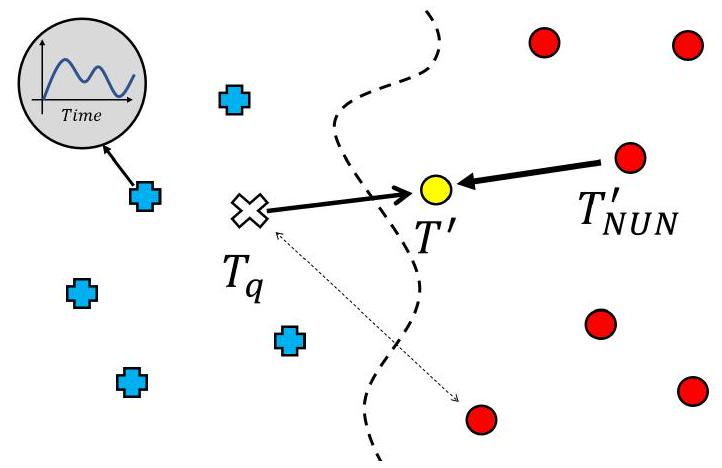
\includegraphics[width=0.4\textwidth]{CF/images/instance-based.jpg}
    \caption{A query time series $T_{q}$ (X with solid arrow) and a nearest-unlike neighbor, $T_{N U N}^{\prime}$ (red circle with solid arrow) are used to guide the generation of counterfactual $T^{\prime}$ (see yellow circle) in a binary classification task. Another in-sample counterfactual (i.e., the next NUN; other red circle with dashed arrow) could also be used to generate another counterfactual for diverse explanations.}
\end{figure}


\textbf{Step 1:} Retrieve native guide. Given a query time series, $T_{q}$, find a counterfactual instance, $T_{\text {Native }}^{\prime}$, that exists in the case-base. An example of one such instance is the query's nearest unlike neighbor $\left(T_{N U N}^{\prime}\right)$. In using these "native counterfactual" cases the method guarantees the explanation's plausibility as it is, by definition, within the distribution. However, such instances are not guaranteed to be sufficiently proximate to the query or, indeed, sparse, so an adaption step is necessary to generate the "explanatory counterfactual", $T^{\prime}$ (see Figure $3)$.

\textbf{Step 2:} Adapt native guide to generate counterfactual. To produce a more proximate explanatory counterfactual, $T^{\prime}$, the native guide, $T_{\text {Native }}^{\prime}$ is perturbed towards the to-be-explained query-case, $T_{q}$ (see Figure 3). Typically, counterfactual methods use some $L_{p}$ distance metric to guide this perturbation (such as Manhattan distance, [55]) and in time series where dynamic time warping (DTW) distance is often more appropriate an analogous averaging technique known as weighted dynamic barycentre averaging can be used 13]. In cases where we are explaining a deep-learner's predictions, the feature-weight vectors of the classifier, $\boldsymbol{\omega}$, can be used to perturb "semantically-meaningful" features of the time series, rather than the "raw" time series data, to guarantee sparsity ${ }^{4}$.
\footnotetext{Note, SHAP can also be used to generate such vectors, if we are directly explaining any given model, rather than twinning.
}

Accordingly, using the feature-weights, the method seeks to modify contiguous, subsequences, rather than the whole time series, as follows:

$$
\begin{aligned}
& T_{q}=\left\{<t_{1}, t_{2}, t_{3}, t_{4}, t_{5} \ldots, t_{n}>\right\} \text { s.t. } b\left(T_{q}\right)=c \\
& T^{\prime}=\left\{<t_{1}, t_{2}^{\prime}, t_{3}^{\prime}, t_{4}^{\prime}, t_{5} \ldots, t_{n}>\right\} \text { s.t. } b\left(T^{\prime}\right)=c^{\prime}
\end{aligned}
$$



\footnotetext{\href{https://github.com/e-delaney/Instance-Based_CFE_TSC}{https://github.com/e-delaney/Instance-Based\_CFE\_TSC}
}

